\PassOptionsToPackage{table}{xcolor}
\documentclass{beamer}
\usepackage[table]{xcolor}
\definecolor{intestazione}{RGB}{220,220,220}
\definecolor{riga1}{RGB}{255,255,255}
\definecolor{riga2}{RGB}{245,245,245}
\graphicspath{ {./images/} }
\usepackage{nameref}
\usetheme{Madrid}

\begin{document}
	
	\title{Gestione centraline elettriche}
	\subtitle{Architettura del software}
	\author{Michele Beccari 856608}
	\date{2024}
	
	\begin{frame}
		\titlepage
	\end{frame}

	\begin{frame}[allowframebreaks]{Indice}
		\tableofcontents
	\end{frame}
	
	
	\section{Obbiettivo del progetto}\label{obbiettivo}
	
	\begin{frame}
		\frametitle{\nameref{obbiettivo}}
		\begin{block}{\nameref{obbiettivo}}
			Si vuole realizzare un sistema per la GEstione di Centraline (GEC) di distribuzione di energia elettrica. \\
			Le centraline sono sparse sul territorio e sono dotate di sensori per la misura istantanea della potenza erogata. \\
			Il sistema deve essere in grado di gestire le anomalie nell'erogazione della potenza delle centraline. \\
			In caso di guasti il sistema deve consentire al servizio tecnico centrale l'invio di un operatore adatto alla risoluzione del guasto.
		\end{block}
	\end{frame}
	
	\section{Assunzioni}\label{assunzioni}
	
	\begin{frame}[allowframebreaks]
		\frametitle{\nameref{assunzioni}}
			\begin{block}{Centraline}
				\begin{itemize}
					\item Possono essere in vari stati (es. centralina attiva, centralina disattivata, centralina pianificata...)
					\item Sono connesse ad internet e quindi possono comunicare con il GEC
					\item Sono dotate di un sensore che consente di leggere la potenza istantanea
					\item Sono dotate di un sistema che ne riceve i dati del sensore ed è in grado di comunicare i dati al servizio tecnico centrale
					\item Possono essere di diverse tipologie
				\end{itemize}
			\end{block}
			\begin{block}{Guasti}
					\begin{itemize}
						\item Ad ogni anomalia viene assegnato un unico operatore per la risoluzione.
						\item Se c'è un guasto in corso per una centralina, tutte le letture anomale fino alla risoluzione del guasto sono considerate causate dall'unico guasto in corso.
					\end{itemize}
			\end{block}
			\begin{block}{Operatori}
				\begin{itemize}
					\item Ogni operatore è in grado di operare su una o più tipologie di centraline.
				\end{itemize}
			\end{block}
			\begin{block}{Politica di distribuzione}
				\begin{itemize}
					\item Una politica di distribuzione è formata da una serie di modifiche alle centraline (aggiunta, modifica, spostamento...)
				\end{itemize}
			\end{block}
			\begin{block}{Dimensioni del problema}
				\begin{itemize}
					\item Il sistema gestisce 500 centraline
					\item Il sistema è supportato da 20 tecnici
					\item Il sistema gestisce 10 guasti giornalieri
				\end{itemize}
			\end{block}
	\end{frame}
	
	\section{Terminologia}\label{terminology}
	
	\begin{frame}
		\frametitle{\nameref{terminology}}
		\begin{block}{Datastore}
			\begin{itemize}
				\item DSC: datastore centraline.
				\item DSG: datastore guasti.
				\item DSLC: datastore letture centraline.
				\item DST: datastore tecnici.
				\item DSI: datastore interventi.
				\item DSPD: datastore politiche di distribuzione.
			\end{itemize}
		\end{block}
		\begin{block}{Buffer}
			\begin{itemize}
				\item BLC: buffer letture centraline.
			\end{itemize}
		\end{block}
	\end{frame}

	\section{Architettura del problema}\label{arch_problema}
	
	
	\subsection{Modello di dominio}\label{domain_model}
	\begin{frame}
		\frametitle{\nameref{domain_model}}
		\begin{center}
			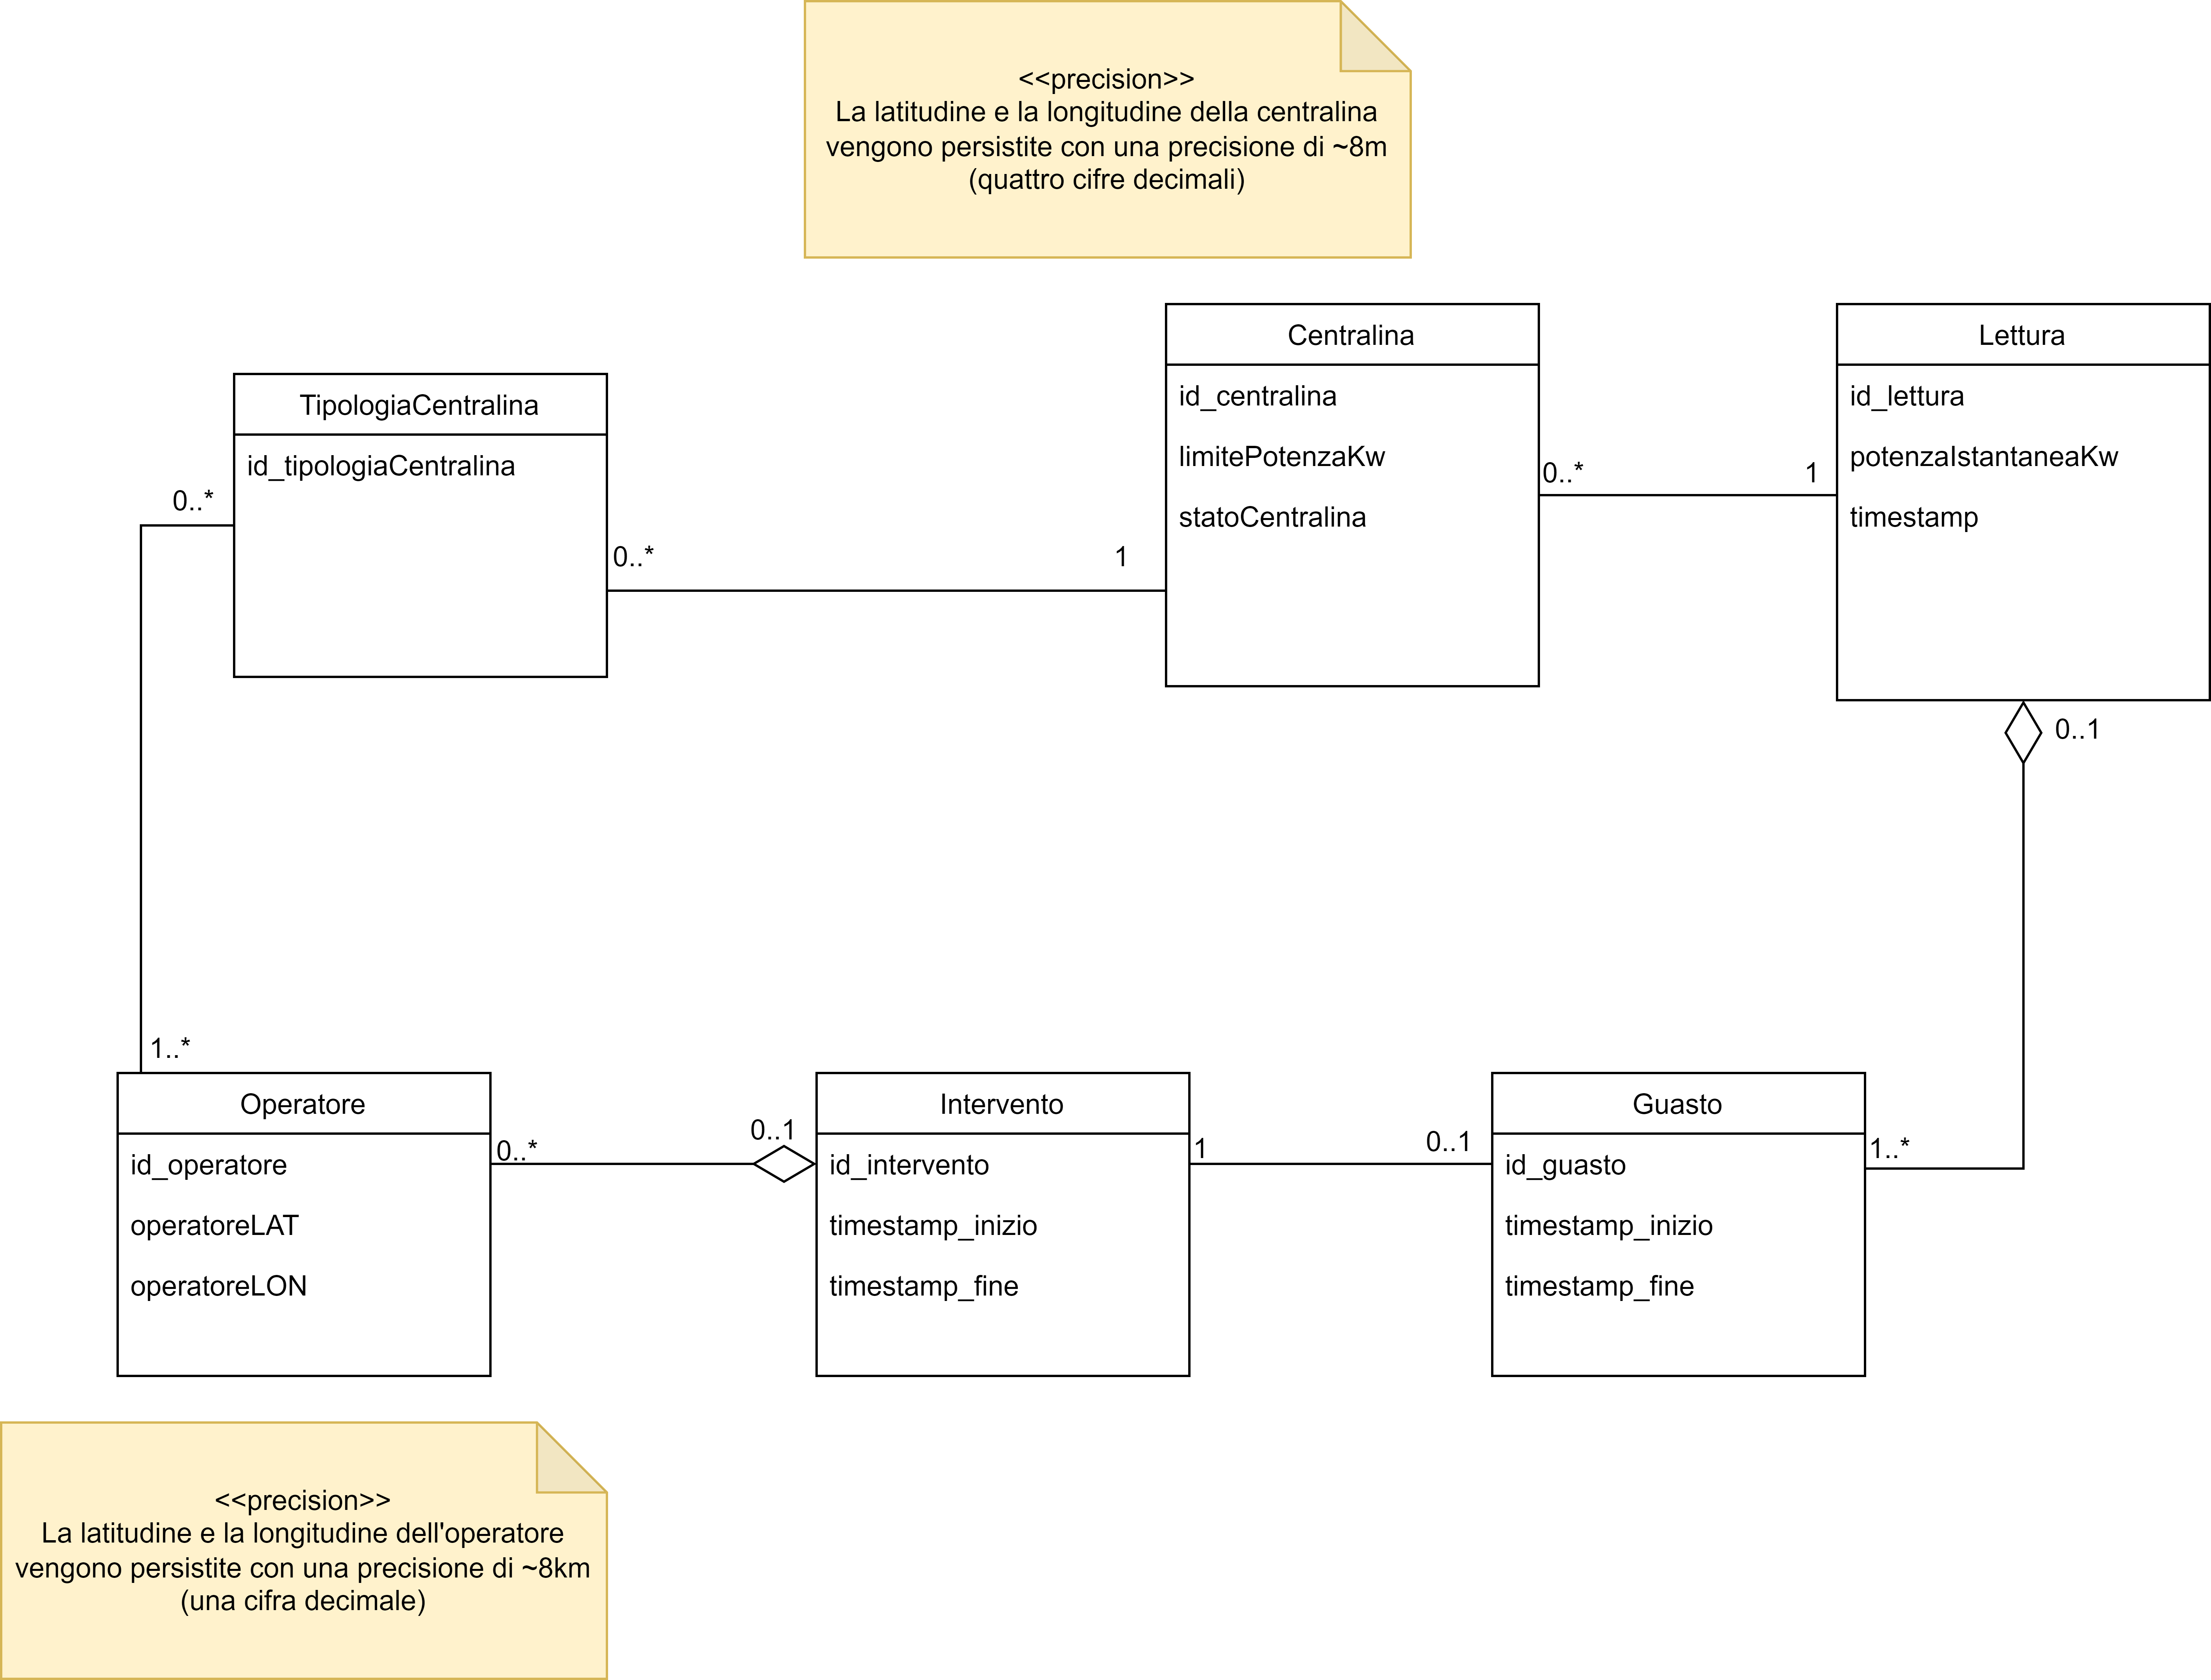
\includegraphics[width=0.85\textwidth, height=\textheight, keepaspectratio=true]{domain_model.png}
		\end{center}
	\end{frame}
	
	\subsection{Diagramma dei casi d'uso}\label{use_cases_diagram}
	\begin{frame}
		\frametitle{\nameref{use_cases_diagram}}
		\begin{center}
			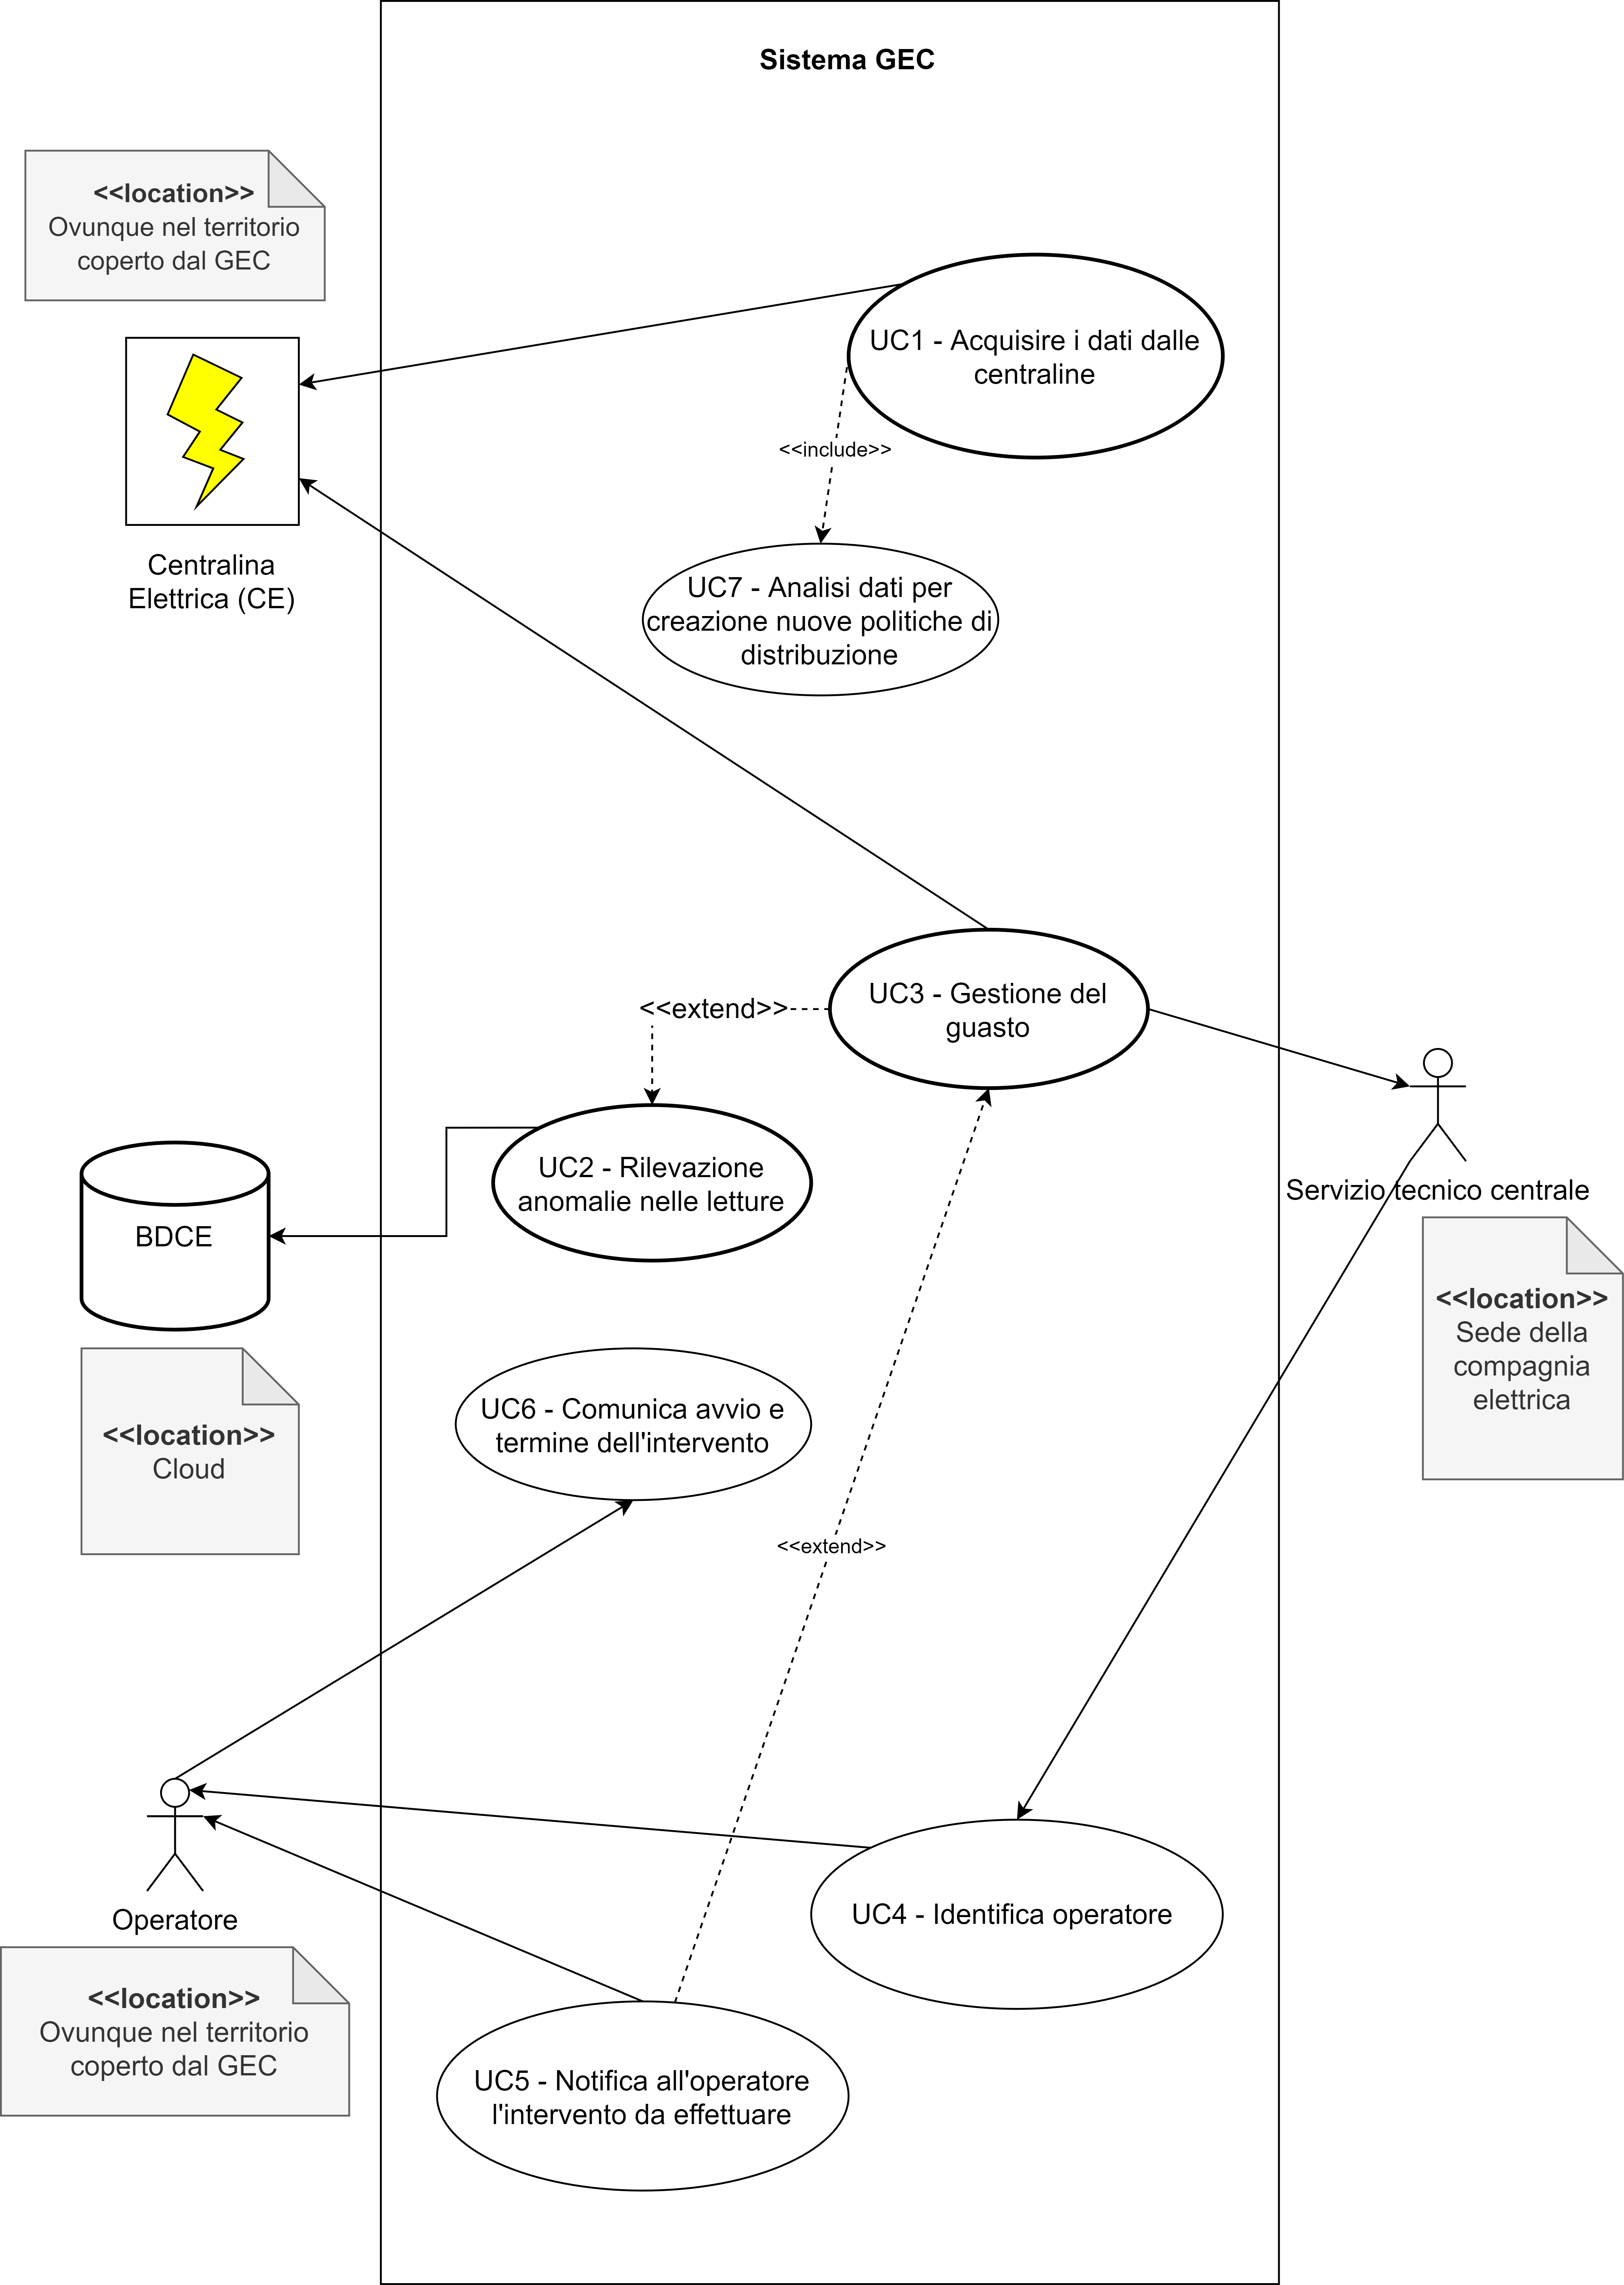
\includegraphics[width=\textwidth, height=0.85\textheight, keepaspectratio=true]{use_cases_diagram.png}
		\end{center}
	\end{frame}

	\subsection{Diagrammi delle attività}\label{activity_diagram}
		\begin{frame}	
		\frametitle{\nameref{use_cases_diagram}}
		\begin{block}{\nameref{use_cases_diagram}}
			\begin{itemize}
				\item ADUC1 - Acquisire dati centraline
				\item ADUC2 - Rilevazione anomalie nelle letture
				\item ADUC3 - Gestione del guasto
				\item ADUC4 - Identifica operatore
				\item ADUC5 - Notifica all'operatore l'intervento da effettuare
				\item ADUC6 - Comunica avvio e termine dell'intervento
				\item ADUC7 - Analisi dati per creazione nuove politiche di distribuzione
			\end{itemize}
		\end{block}
		\end{frame}
		
		\begin{frame}
	    \subsubsection{ADUC1 - Acquisire dati centraline}	 
		\begin{block}{ADUC1 - Acquisire dati centraline}
			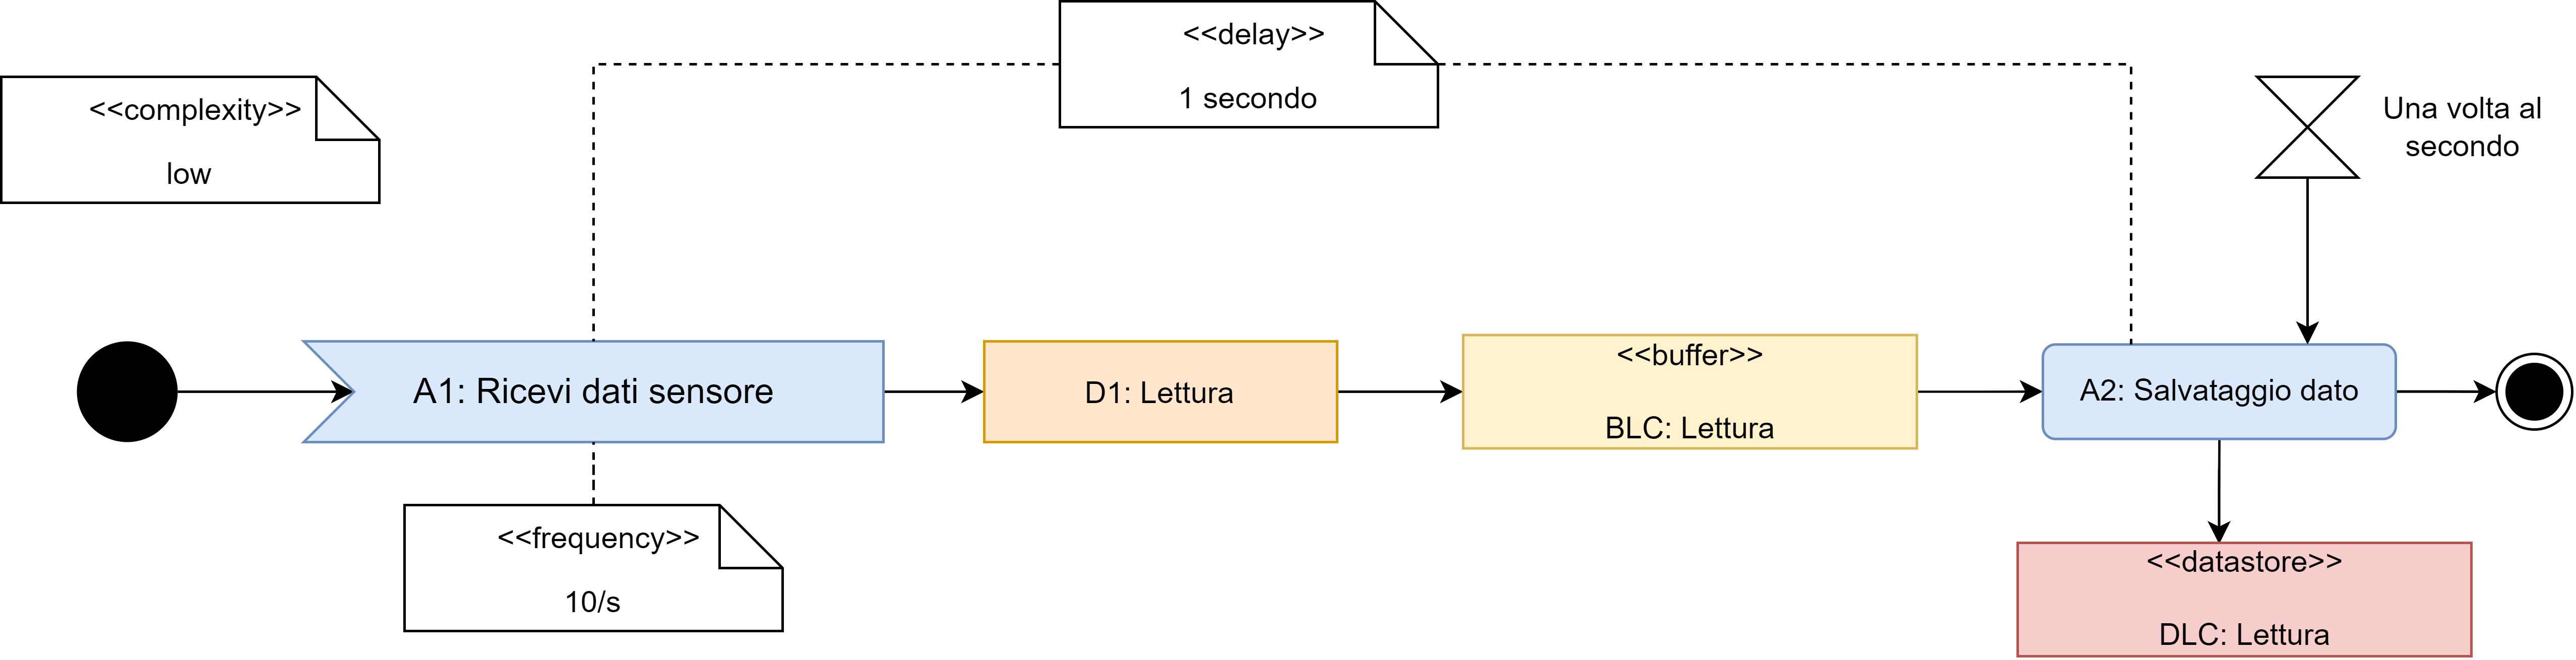
\includegraphics[width=\textwidth, height=0.85\textheight, keepaspectratio=true]{ADUC1.png}
		\end{block}
		\end{frame}

		
		\begin{frame}
		\subsubsection{ADUC2 - Rilevazione anomalie nelle letture}		
		\begin{block}{ADUC2 - Rilevazione anomalie nelle letture}
			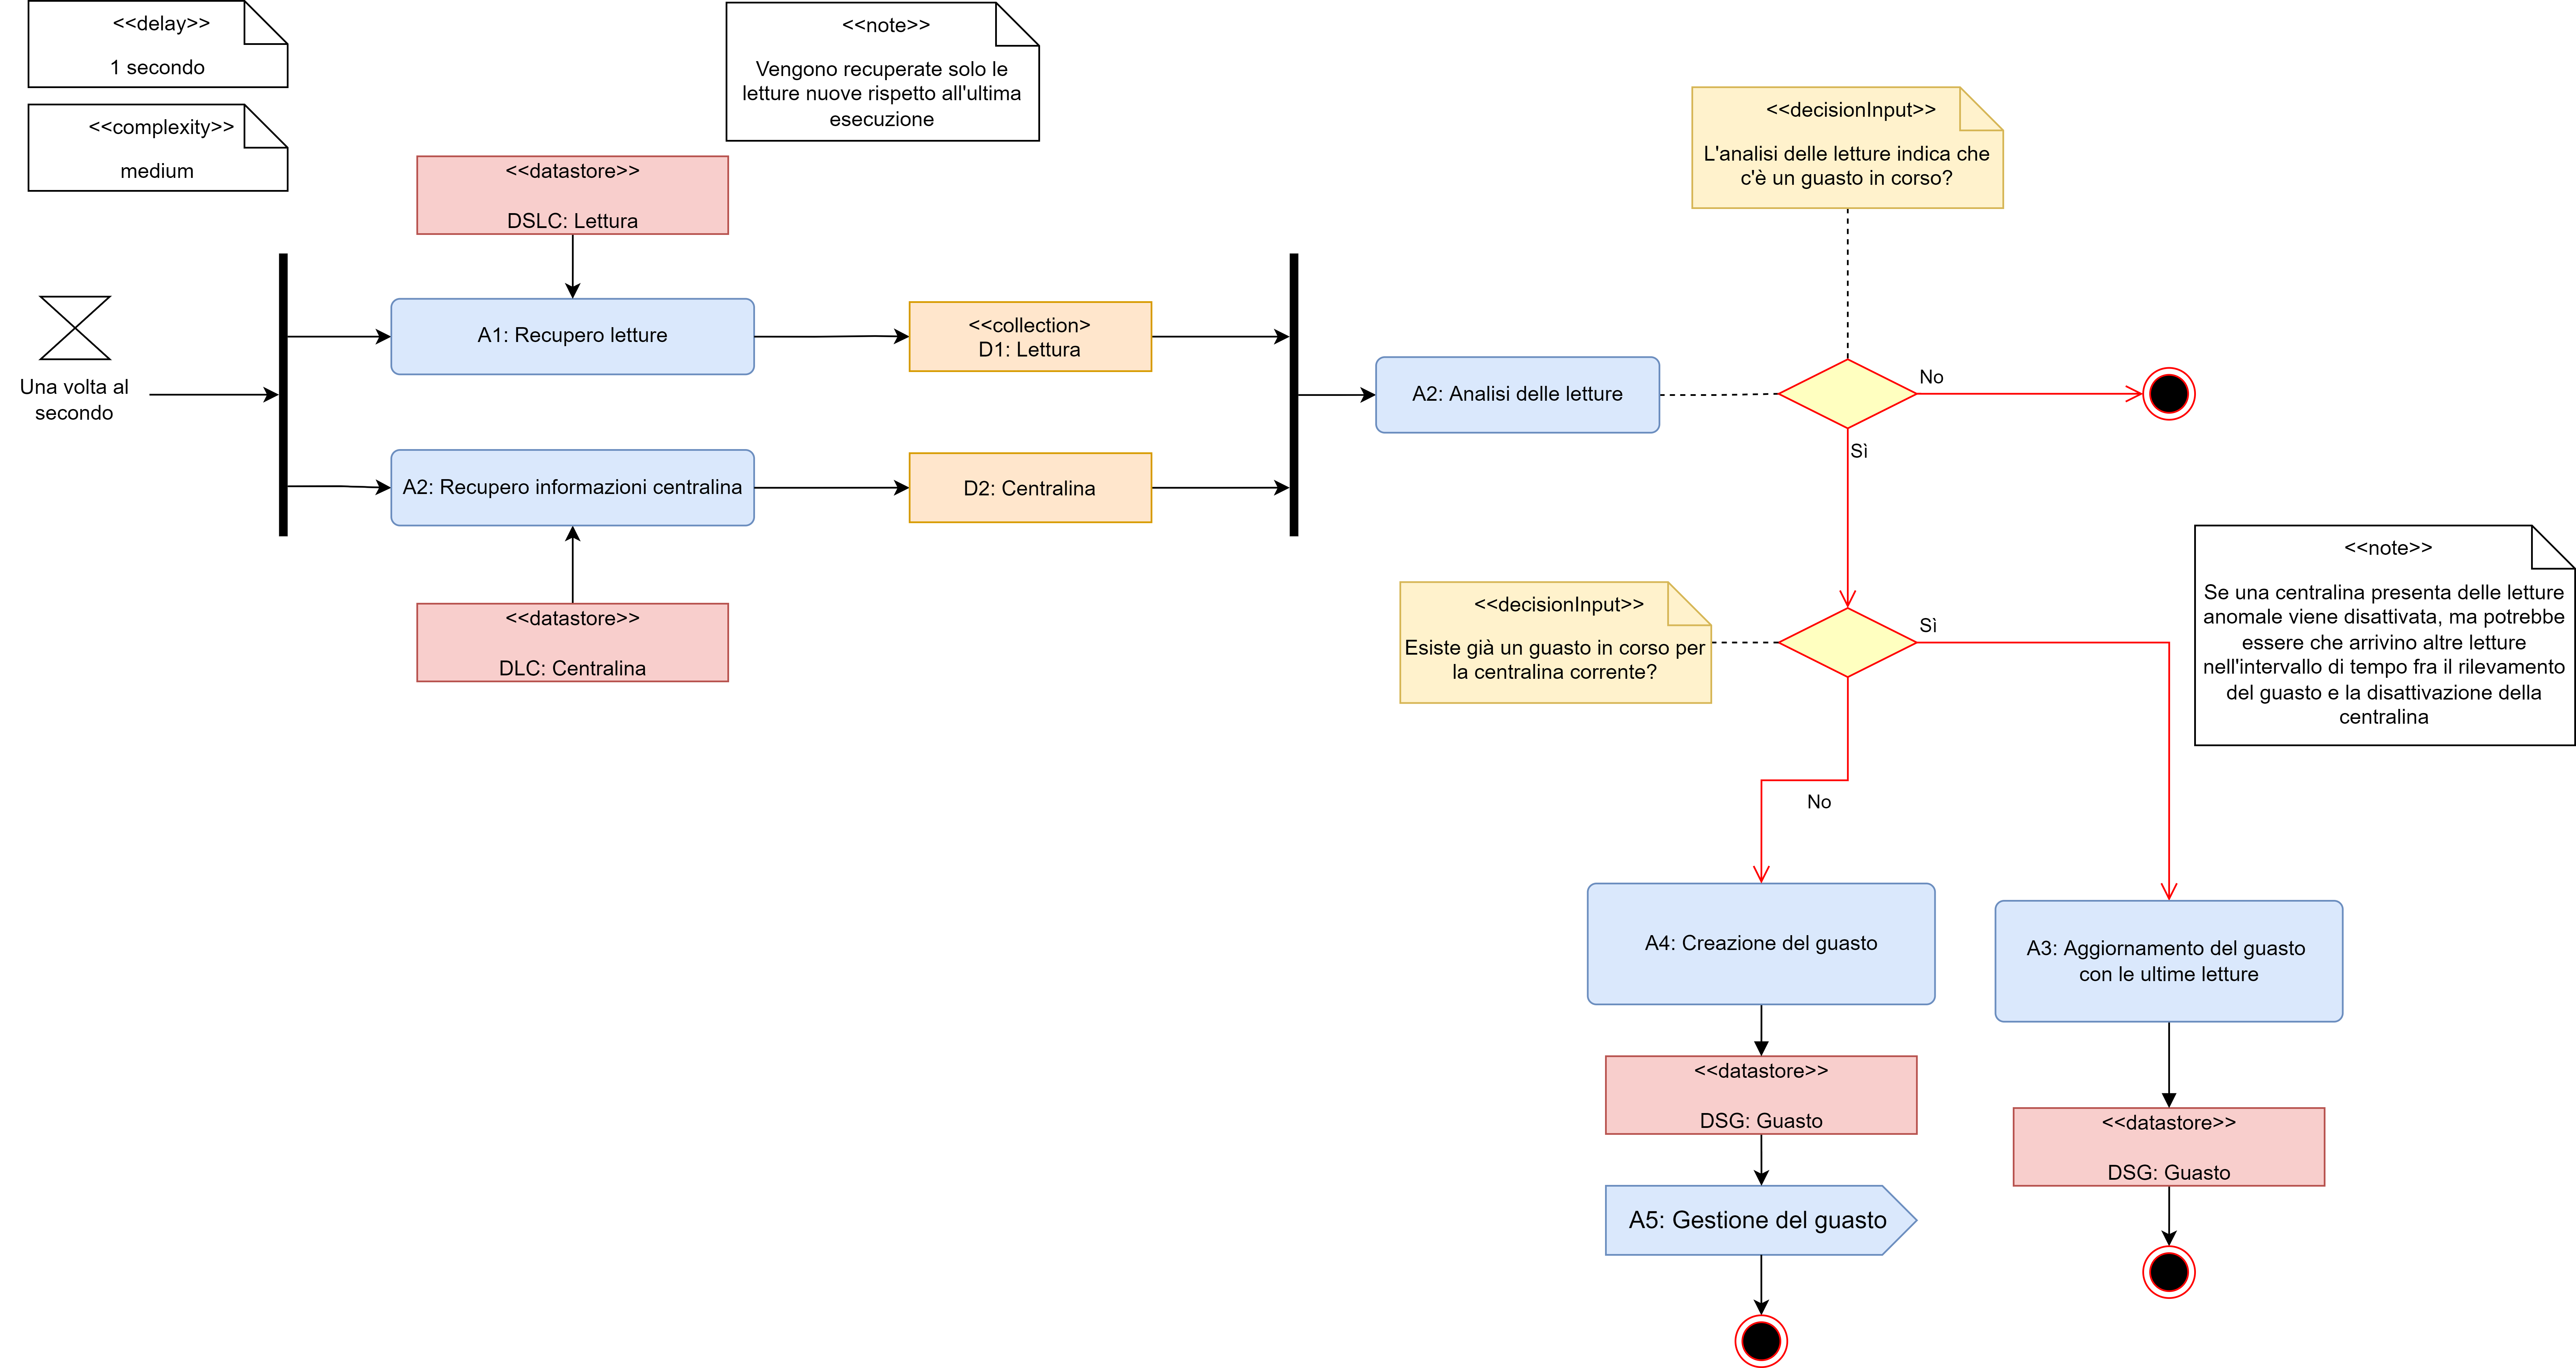
\includegraphics[width=\textwidth, height=0.85\textheight, keepaspectratio=true]{ADUC2.png}
		\end{block}
		\end{frame}

	
		\begin{frame}
		\subsubsection{ADUC3 - Gestione del guasto}	
			\begin{block}{ADUC3 - Gestione del guasto}
				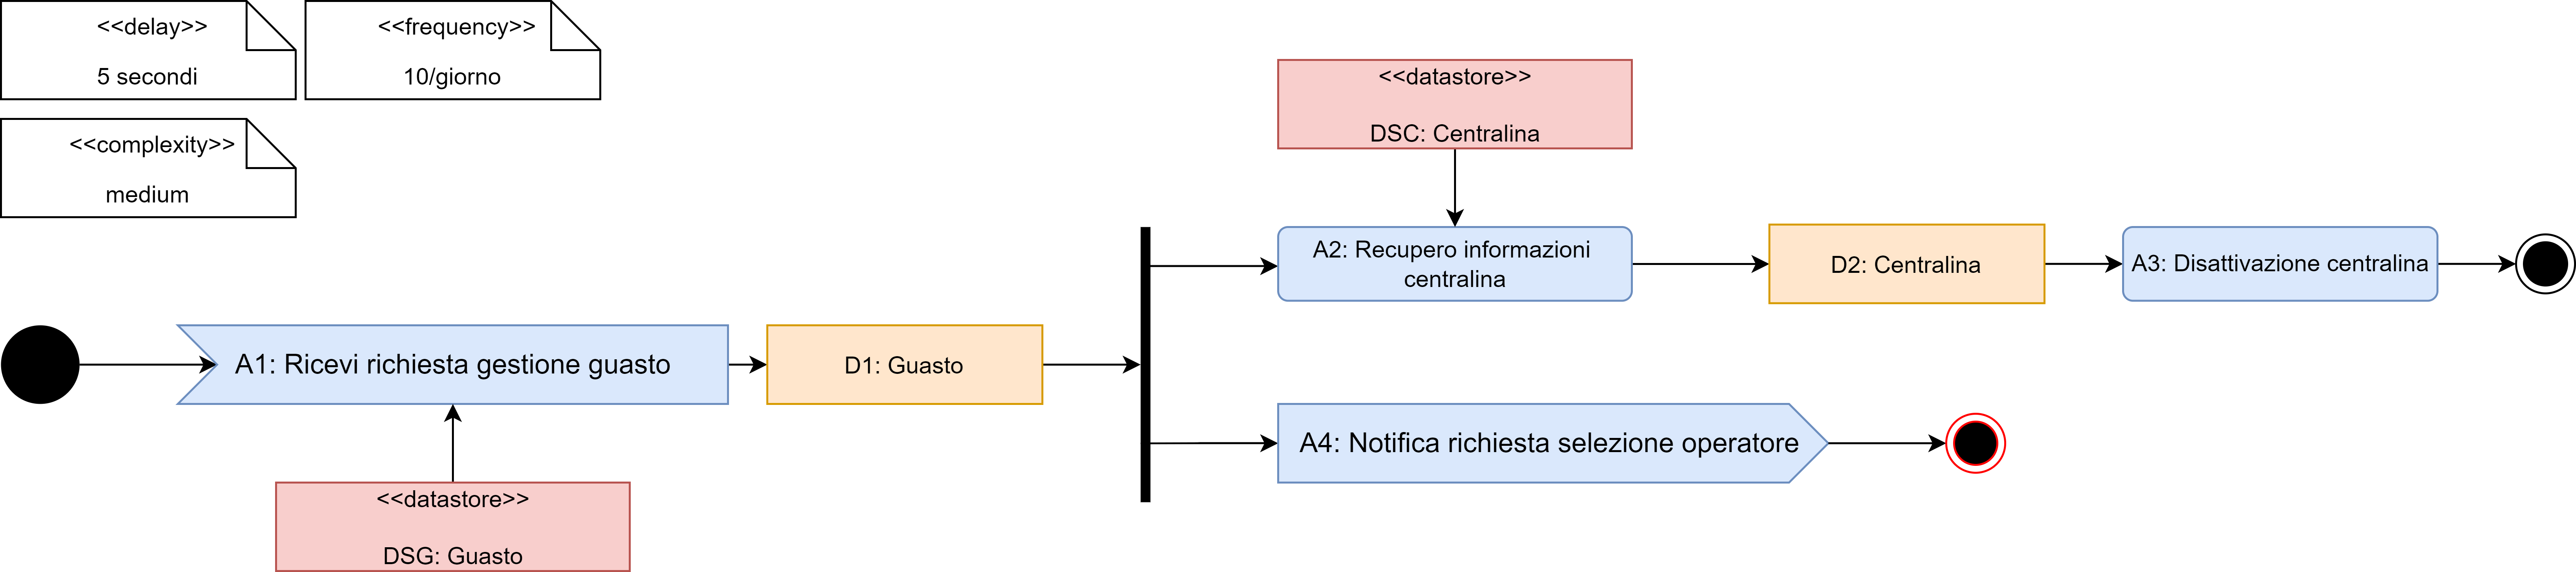
\includegraphics[width=\textwidth, height=0.85\textheight, keepaspectratio=true]{ADUC3.png}
			\end{block}
		\end{frame}
	
		\begin{frame}
		\subsubsection{ADUC4 - Identifica operatore}	
			\begin{block}{ADUC4 - Identifica operatore}
				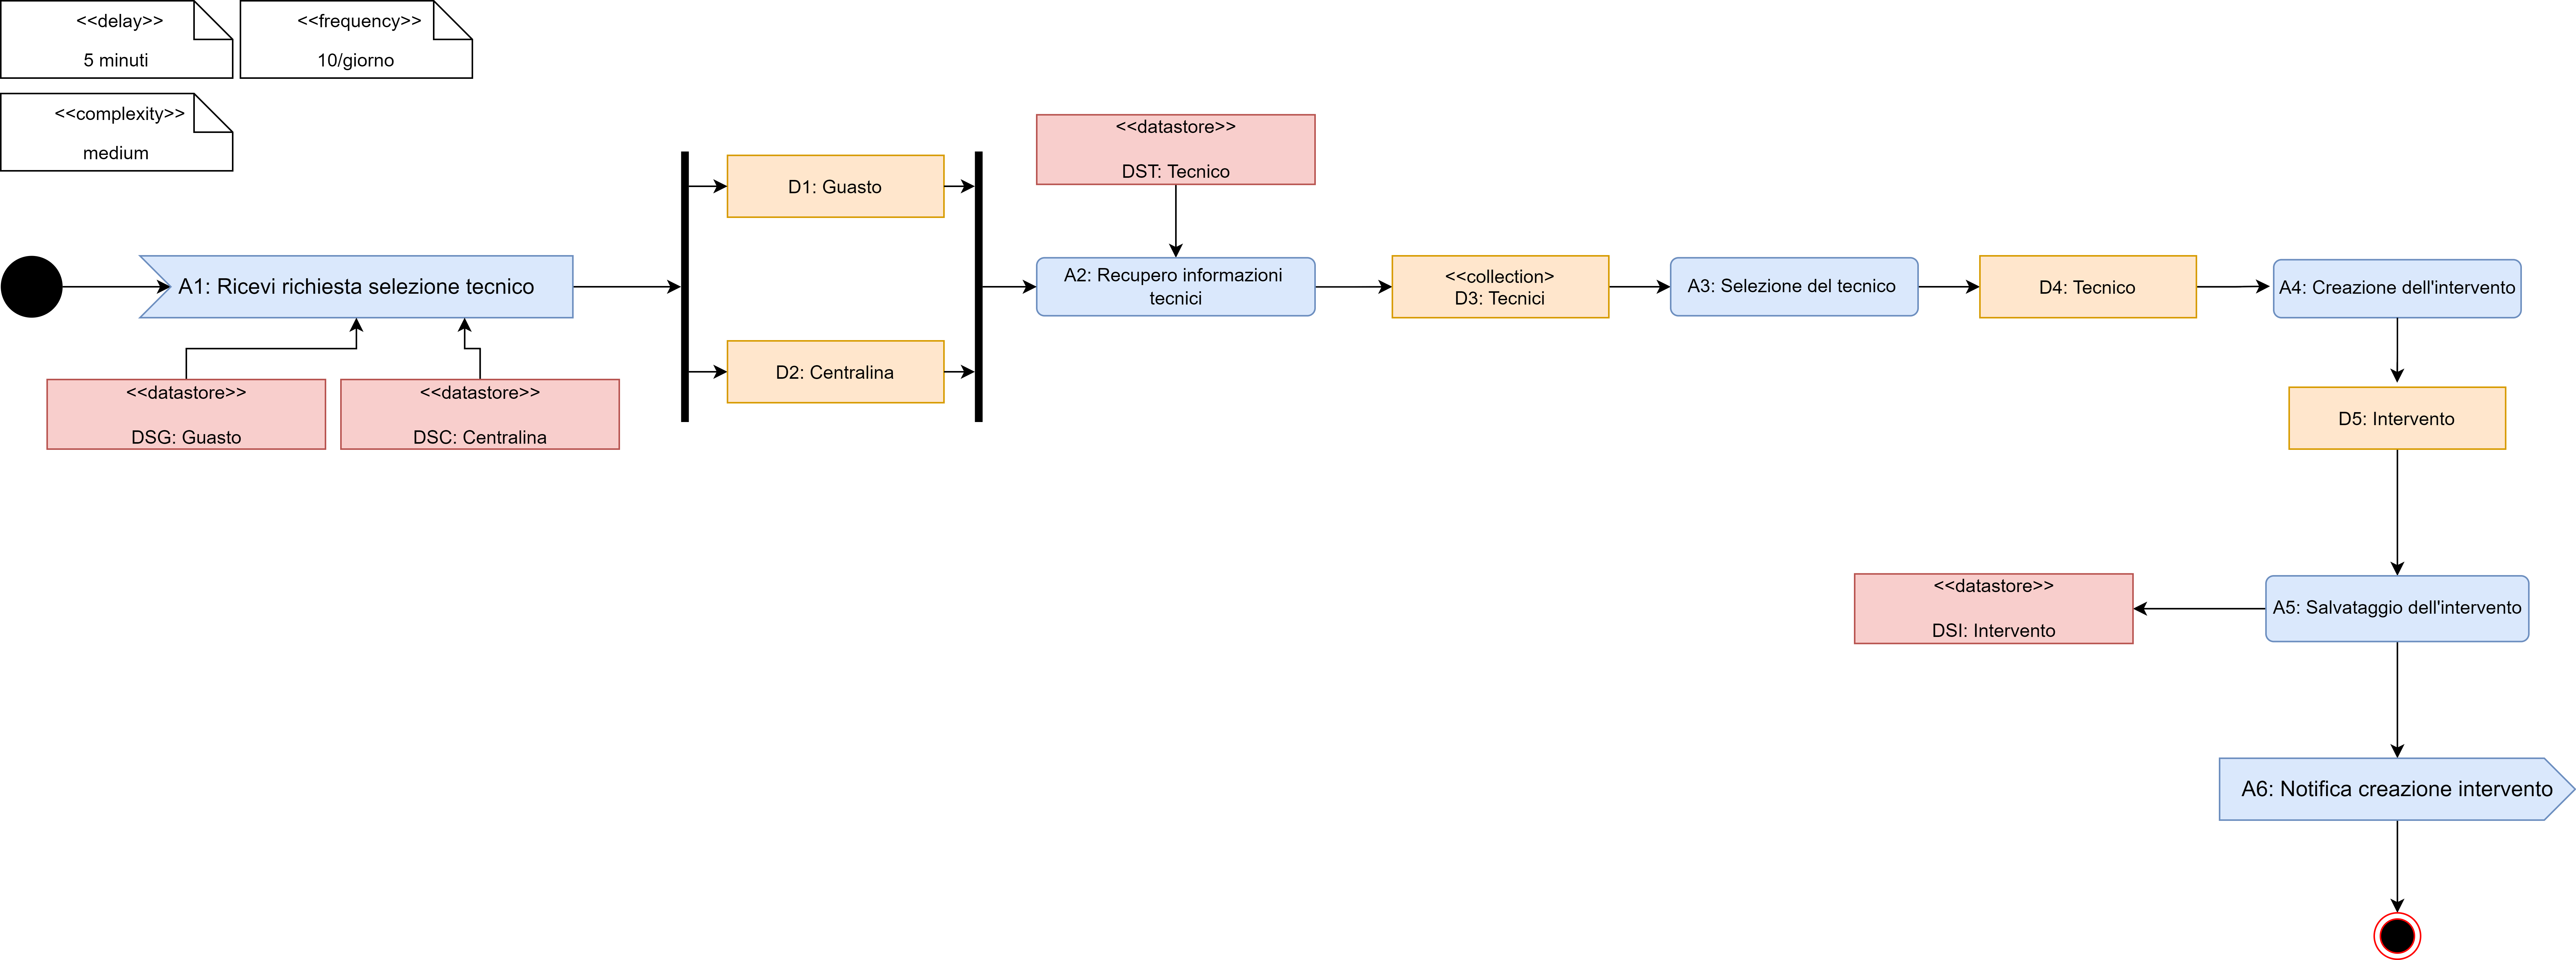
\includegraphics[width=\textwidth, height=0.85\textheight, keepaspectratio=true]{ADUC4.png}
			\end{block}
		\end{frame}

		\begin{frame}
		\subsubsection{ADUC5 - Notifica all'operatore}	
			\begin{block}{ADUC5 - Notifica all'operatore l'intervento da effettuare}
				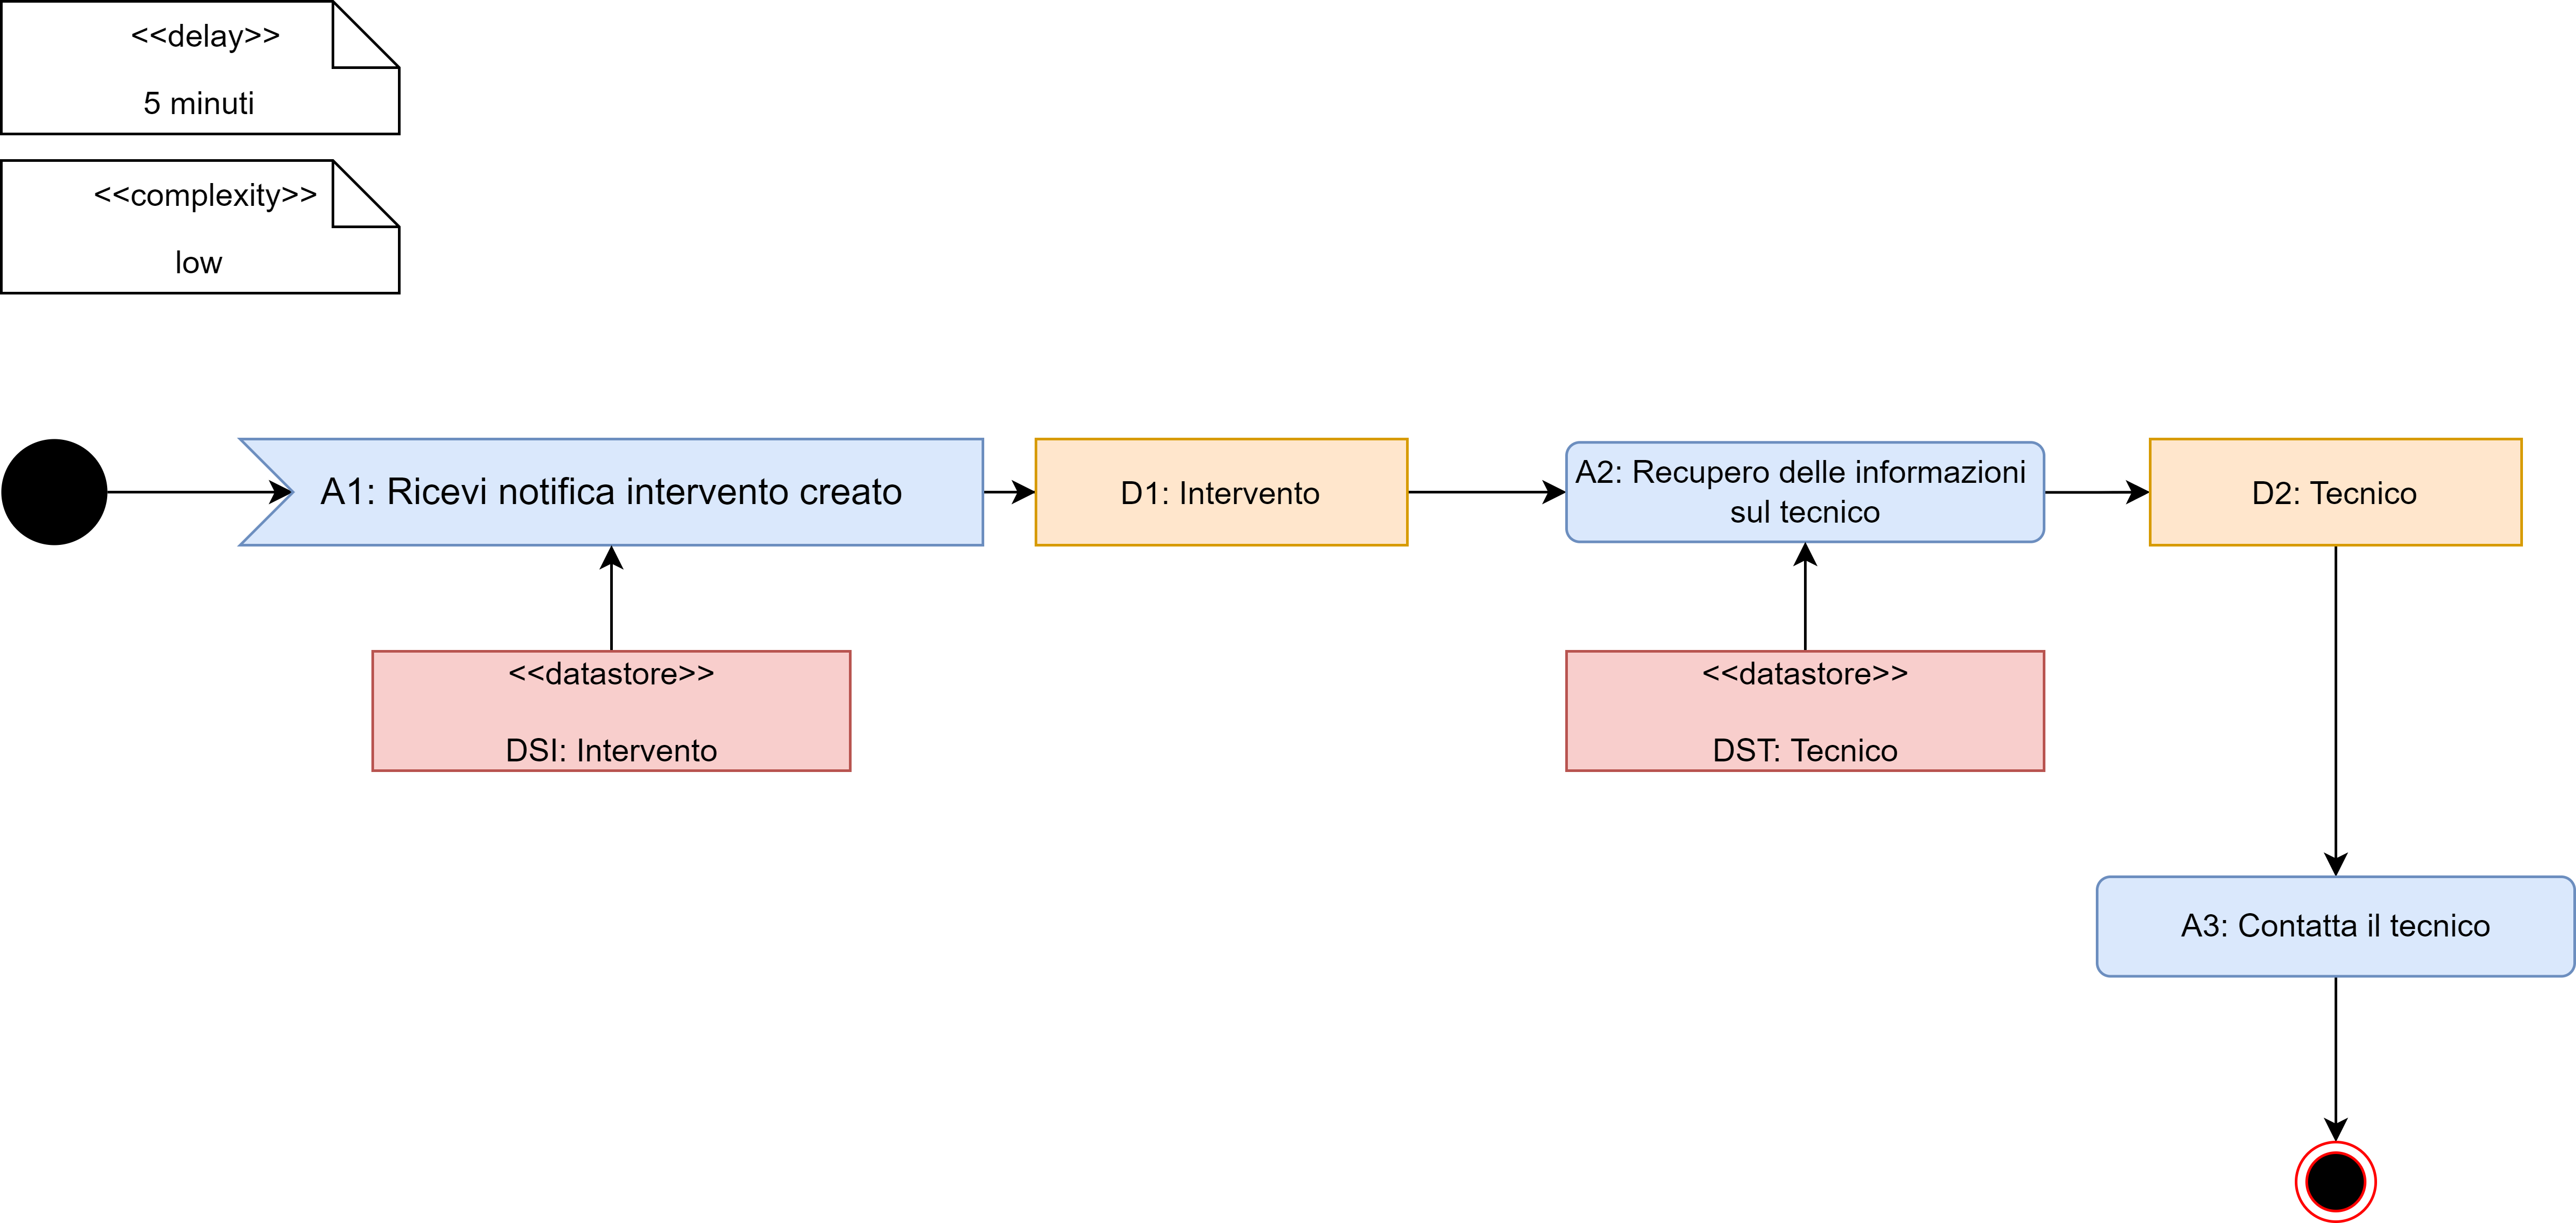
\includegraphics[width=\textwidth, height=0.85\textheight, keepaspectratio=true]{ADUC5.png}
			\end{block}
		\end{frame}	

		\begin{frame}
		\subsubsection{ADUC6 - Comunica avvio e termine dell'intervento}			
			\begin{block}{ADUC6 - Comunica avvio e termine dell'intervento}
				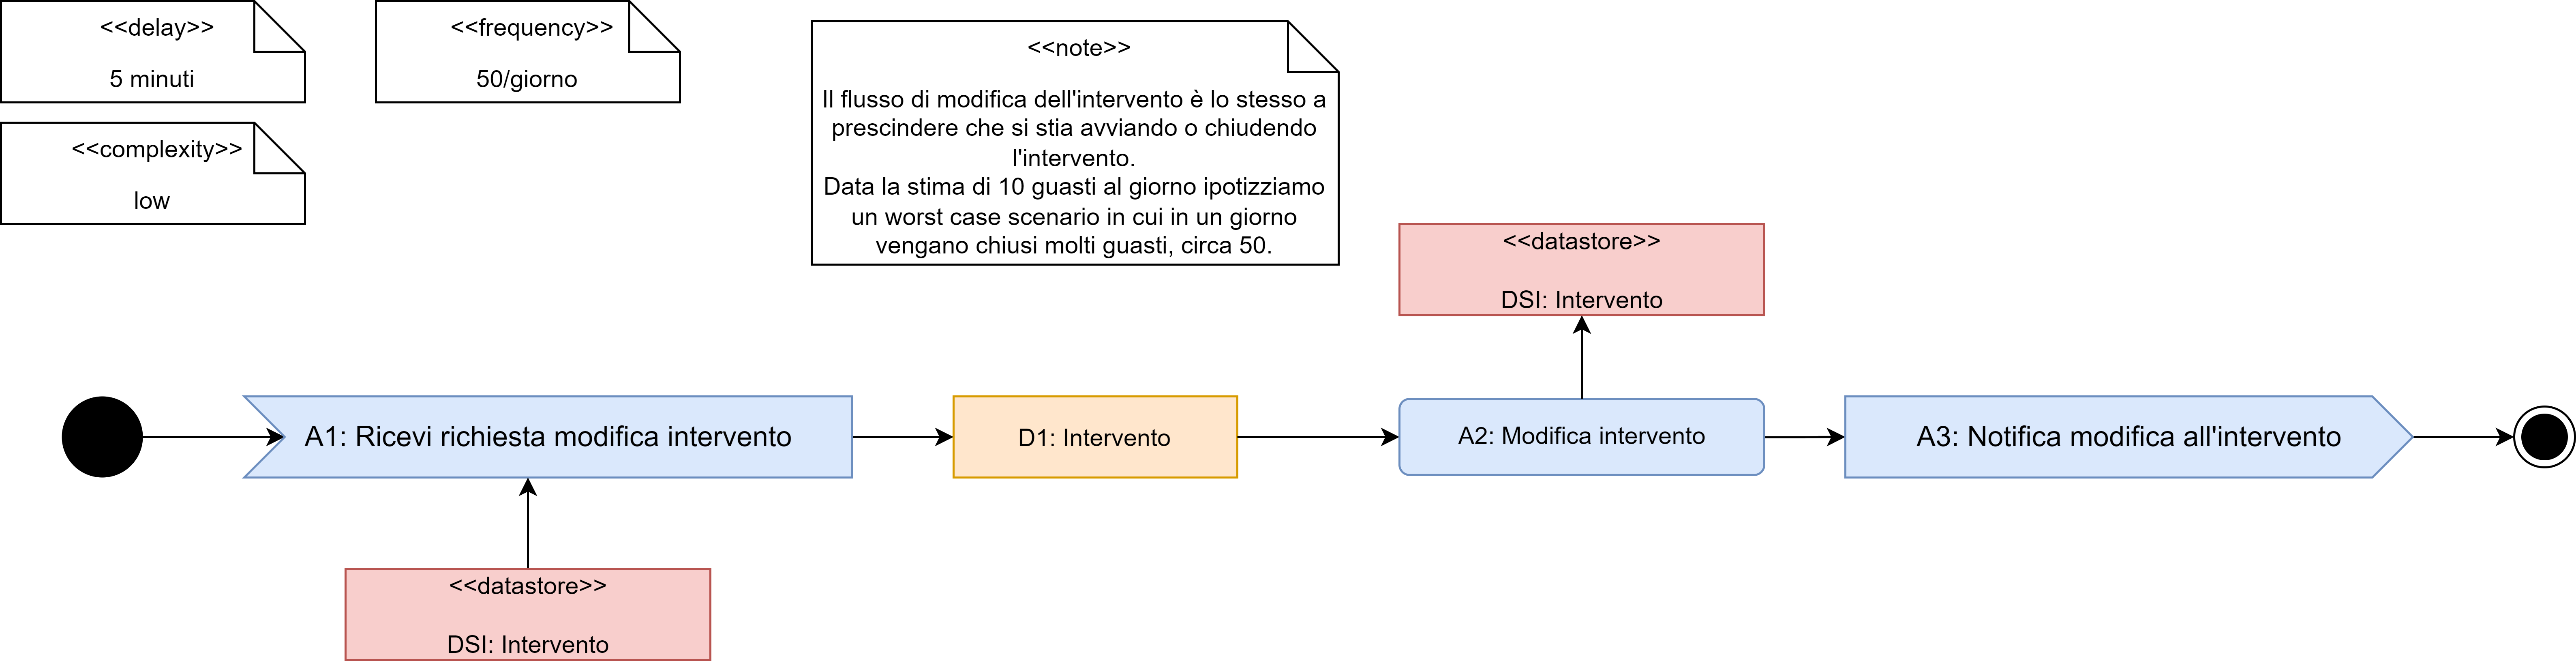
\includegraphics[width=\textwidth, height=0.85\textheight, keepaspectratio=true]{ADUC6.png}
			\end{block}
		\end{frame}	
	
		\begin{frame}
		\subsubsection{ADUC7 - Analisi dati per creazione nuove politiche di distribuzione}			
			\begin{block}{ADUC7 - Analisi dati per creazione nuove politiche di distribuzione}
				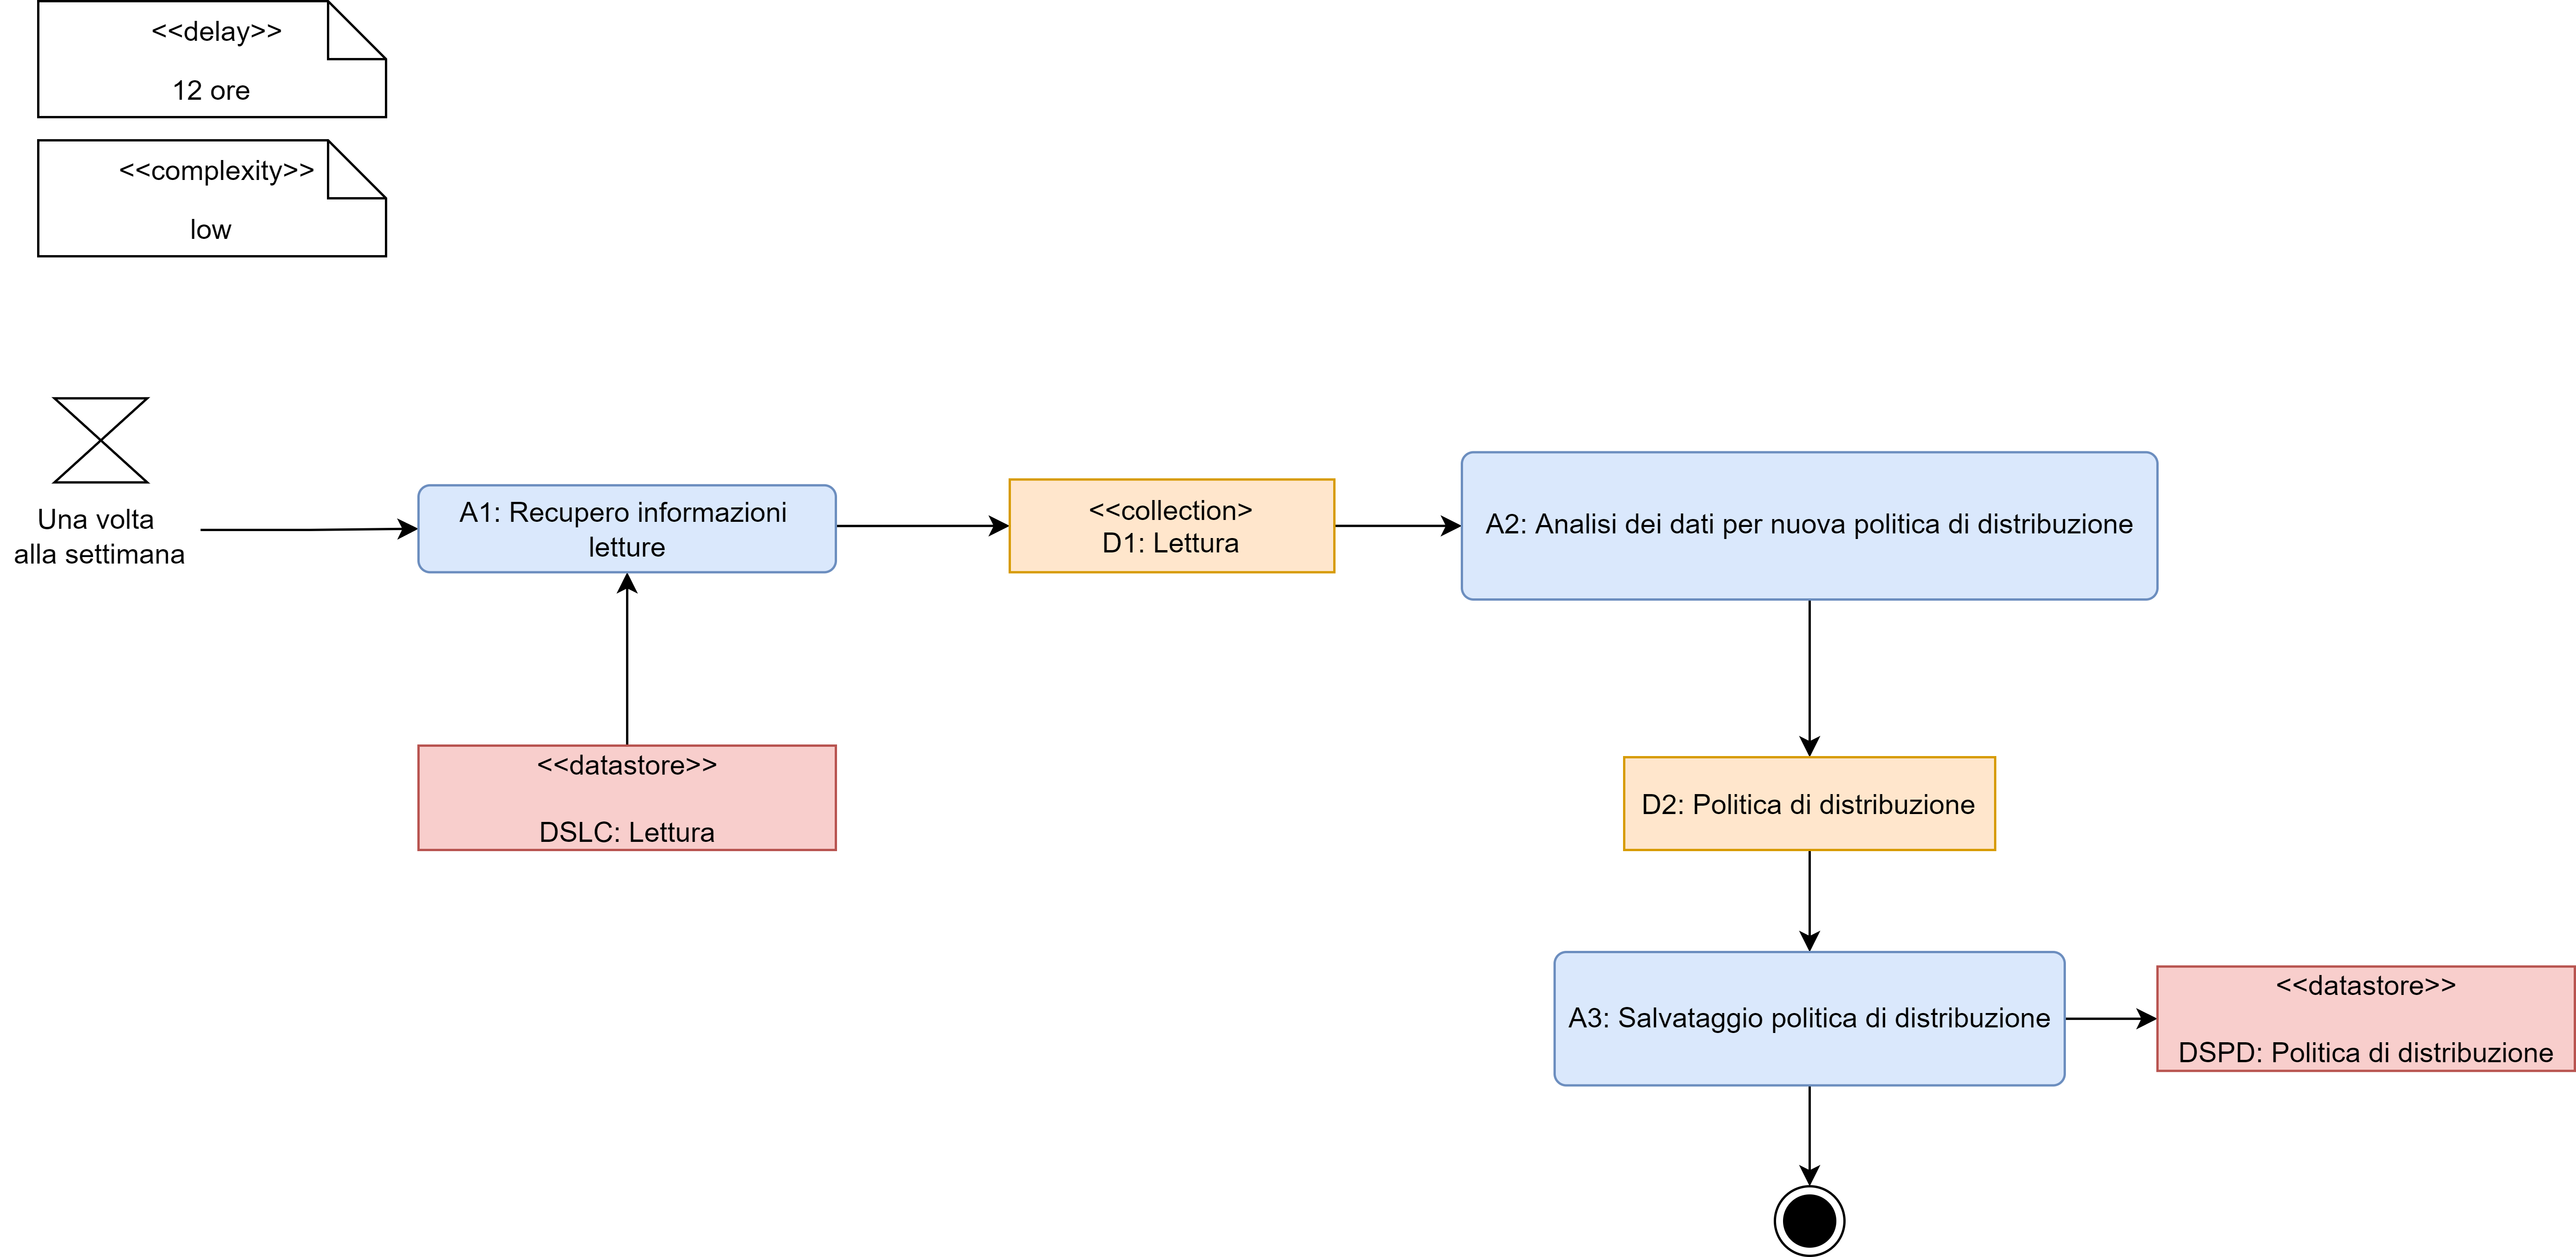
\includegraphics[width=\textwidth, height=0.85\textheight, keepaspectratio=true]{ADUC7.png}
			\end{block}
		\end{frame}	
	
	\section{Architettura logica}
	\subsection{Valori dimensionali architetturali strutturali}\label{val_dim_arch_strut}
	
	\begin{frame}
		\frametitle{\nameref{val_dim_arch_strut}}			
		\begin{center}
				\begin{table}
				\centering
				\begin{tabular}{|c|c|c|}
					\hline
					\rowcolor{intestazione}
					Dimensione & Valori ammissibili & \#Valori ammissibili \\
					\hline
					\rowcolor{riga1}
					Complessità & low, low & 2 \\
					\rowcolor{riga2}
					Frequency & 10/s, 1/s, 10/giorno, 50/giorno, 1/settimana & 5 \\
					\rowcolor{riga1}
					Delay & 1s, 5s, 5 minuti, 12 ore & 4e \\
					\rowcolor{riga2}
					Dato 10 & Dato 11 & Dato 12 \\
					\rowcolor{riga1}
					Dato 13 & Dato 14 & Dato 15 \\
					\rowcolor{riga2}
					Dato 16 & Dato 17 & Dato 18 \\
					\hline
				\end{tabular}
			\end{table}
		\end{center}

	\end{frame}	
	
\end{document}
